\documentclass[11pt]{article}
\usepackage[margin=2.2cm]{geometry}
\usepackage{graphicx}
\usepackage{booktabs}
\usepackage{amsmath,amssymb}
\usepackage{placeins}
\usepackage{needspace}
\usepackage[hidelinks]{hyperref}
\setlength{\parskip}{0.4em}
\setlength{\emergencystretch}{3em}
\makeatletter\setlength{\@fptop}{0pt}\makeatother   % float pages start at the top
\graphicspath{{figures/}}

\title{Dutta E91-013: integrals of the (e,e$'$p) spectral-function data}
\author{Liang Liu}
\date{\today}

\begin{document}
\maketitle

Summary of what the author data tables behind the Dutta \emph{et al.} JLab
Hall~C \textbf{E91-013} paper
(\href{https://arxiv.org/abs/nucl-ex/0303011}{nucl-ex/0303011}, \texorpdfstring{$^{12}$C}{C12} /
\texorpdfstring{$^{56}$Fe}{Fe56} / $^{197}$Au quasi-elastic (e,e$'$p)) integrate to, and on which
scale. This document is the write-up that goes with \texttt{integrate\_dutta.py}
(the integrator) and \texttt{make\_published\_vs\_table.py} (the published-vs-table
figures of section~1); it is generated by \texttt{make\_report\_tex.py} from the
same data files as the markdown version (\texttt{README.md}).

\begin{itemize}
\item Paper source: \texttt{papers/nucl-ex\_0303011/} (tex \texttt{longpaper2.tex};
  every \texttt{tex:line} below anchors to it); published figure renders in
  \texttt{papers/nucl-ex\_0303011/figures/}.
\item Author data: \texttt{data/Dipingkar-dutta-data-prc\_figs/} --- 14 files,
  exactly figs~6, 7, 9, 11 of the paper.
\item Earlier per-figure report: \texttt{report/\allowbreak dutta-e91013-figures.md}. Its
  normalization reading of figs~9/11 (``$\approx Z$, full-occupancy scale'')
  is the old one; the sections after section~1 here supersede it.
\end{itemize}

Sections 4 (the conventions behind the factor $\tfrac12$ and the
positive-half 3D integral; nucleon counts against $T \cdot Z / f_\mathrm{corr}$)
and 5 (windowed integrals, shell occupancies, caveats) are still to be
written.

\section{\texorpdfstring{$E_m$ and $p_m$}{Em and pm} for C12 and Fe56: each published figure next to its data table}

\subsection{The four figures, published vs table}

Left: the paper's render (autocropped). Right: the same quantity drawn from
the \texttt{.dat} files on the paper's axes --- points with the tabulated
statistical errors, \textbf{no rescaling} (no $\tfrac12$ on the $E_m$ files,
no L+R fold on the $p_m$ files; those conventions are the subject of the next
sections). The $p_m$ replots use the house colour cycle with fig~6's marker
shapes per $Q^2$ (fig~7 in print assigns markers differently; the legends
identify the sets). Numbers quoted below come from
\texttt{dutta\_published\_vs\_table.txt}: a per-file ratio to the $Q^2 = 1.8$
reference and a histdiag \texttt{describe1d} readout of all 14 files,
computed on the tabulated values.

\paragraph{\texorpdfstring{$^{12}$C}{C12} missing energy (fig~9).}
The 16 tabulated points are the published ones: $0.571 \pm 0.005$ MeV$^{-1}$
at $E_m = 17.5$ MeV, 0.269 at 22.5, the s-shell bump peaking at 0.077 at
37.5, and three exact zeros below 15 MeV. The IPSM curve exists only in
print. The one visible difference is the error bars: the file's column~4 is
statistical (0.8\,\% at the peak), while the published bars at 17.5 and
22.5 MeV are several times larger (pixel-measured in
\texttt{dutta-e91013-figures.md} \S5).

\begin{figure}[htbp]
\centering
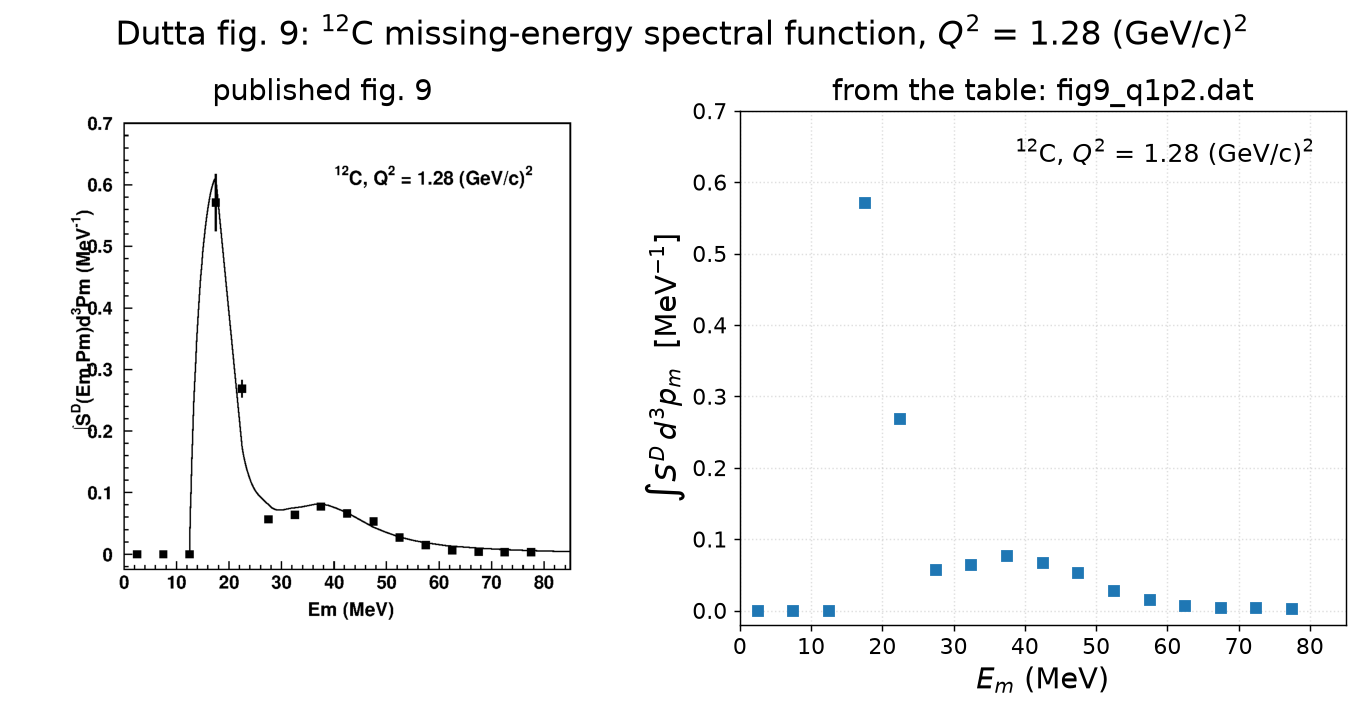
\includegraphics[width=\textwidth]{dutta_fig9_c12_em_published_vs_table.png}
\caption{Fig.~9 of the paper (left) and the 16 points of \texttt{fig9\_q1p2.dat} (right).}
\end{figure}

\paragraph{\texorpdfstring{$^{12}$C}{C12} missing momentum, p-shell and s-shell windows (fig~6).}
Three of the four $Q^2$ sets sit on the published points: relative to the
$Q^2 = 1.8$ reference file the bin-wise median ratio is 1.01 ($Q^2 = 1.28$)
and 0.97 (3.25) in the p-shell panel, 1.14 and 1.20 in the s-shell panel,
with the signed-axis sums equal to within 5--8\,\%. The \textbf{$Q^2 = 0.64$
files do not}: their median ratio to the reference is 1.27 (p-shell) and
1.33 (s-shell) with a $p_m$-dependent spread (1.07--1.44), whereas in print
all four $Q^2$ coincide within marker size. Those two files are excluded from
every integral in this document (open question tracked in
\texttt{open\_questions.md}). The $\ell = 1$ dip at $p_m = 0$ in the p-shell
window and the $\ell = 0$ peak in the s-shell window (tex:920--922) are in
the tables as printed: in the $Q^2 = 1.28$ file the p-shell dip bin is 0.31 of
its peak at $|p_m| = 100$ MeV/c.

\begin{figure}[htbp]
\centering
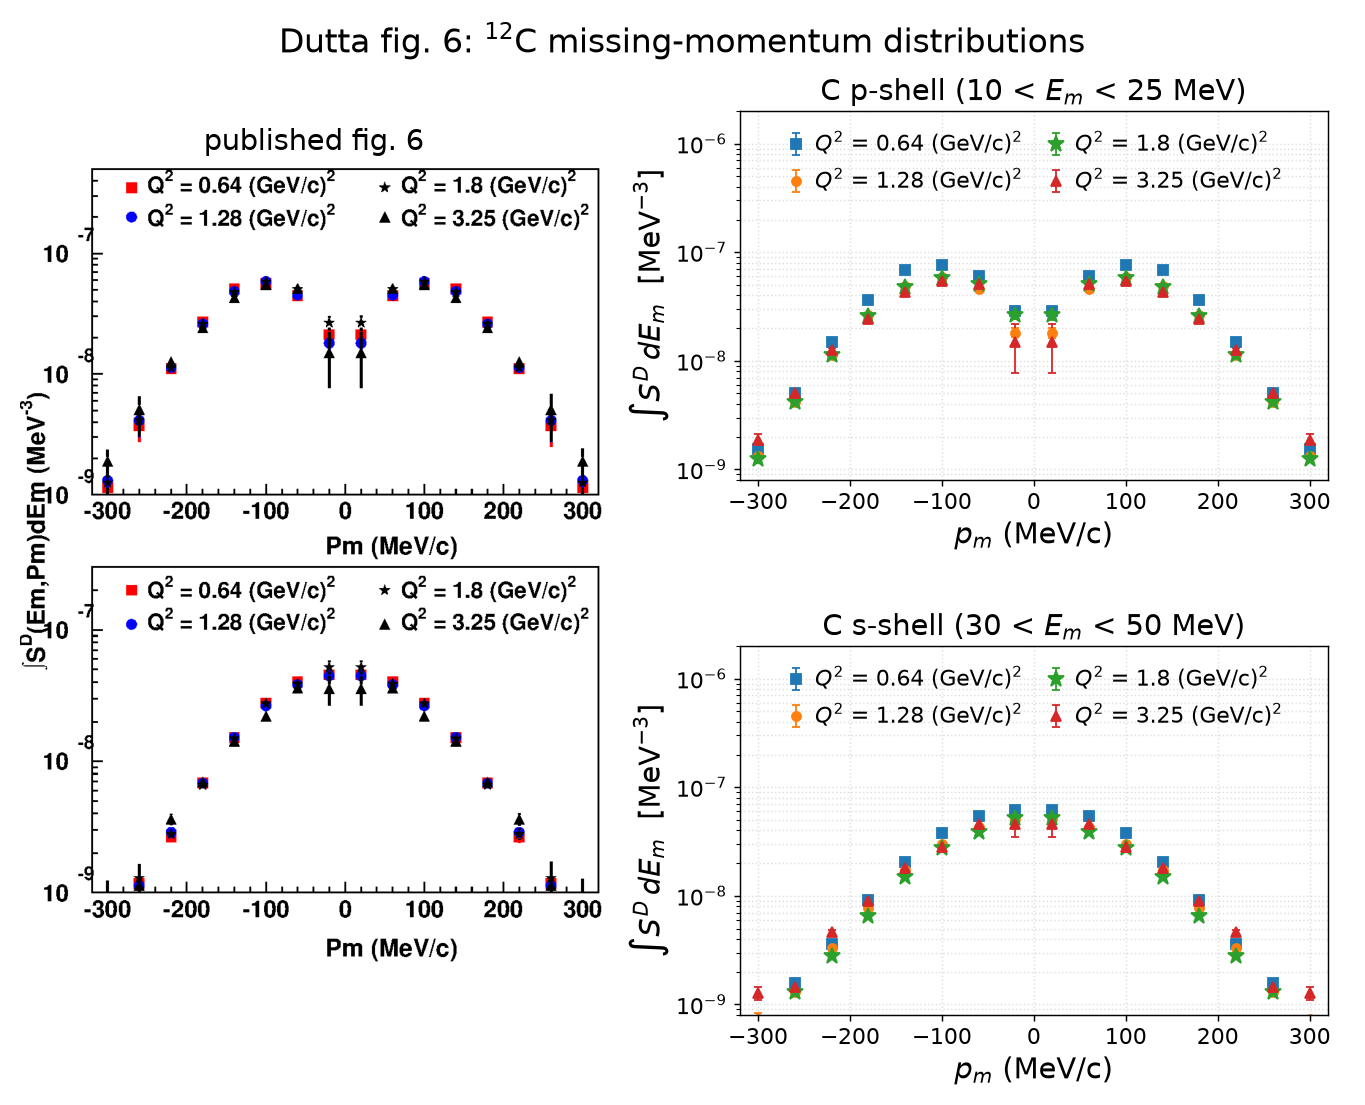
\includegraphics[width=\textwidth]{dutta_fig6_c12_pm_published_vs_table.png}
\caption{Fig.~6 of the paper (left) and the eight \texttt{fig6\_*.dat} files (right), four $Q^2$ sets per panel.}
\end{figure}

\paragraph{\texorpdfstring{$^{56}$Fe}{Fe56} missing energy (fig~11).}
The table reproduces the published points ($0.810 \pm 0.009$ MeV$^{-1}$ at
$E_m = 12.5$ MeV, then a monotone fall to 0.055 at 77.5; two exact zeros
below 10 MeV). The three theory curves (IPSM, Benhar, TIMORA) exist only in
print.

\begin{figure}[htbp]
\centering
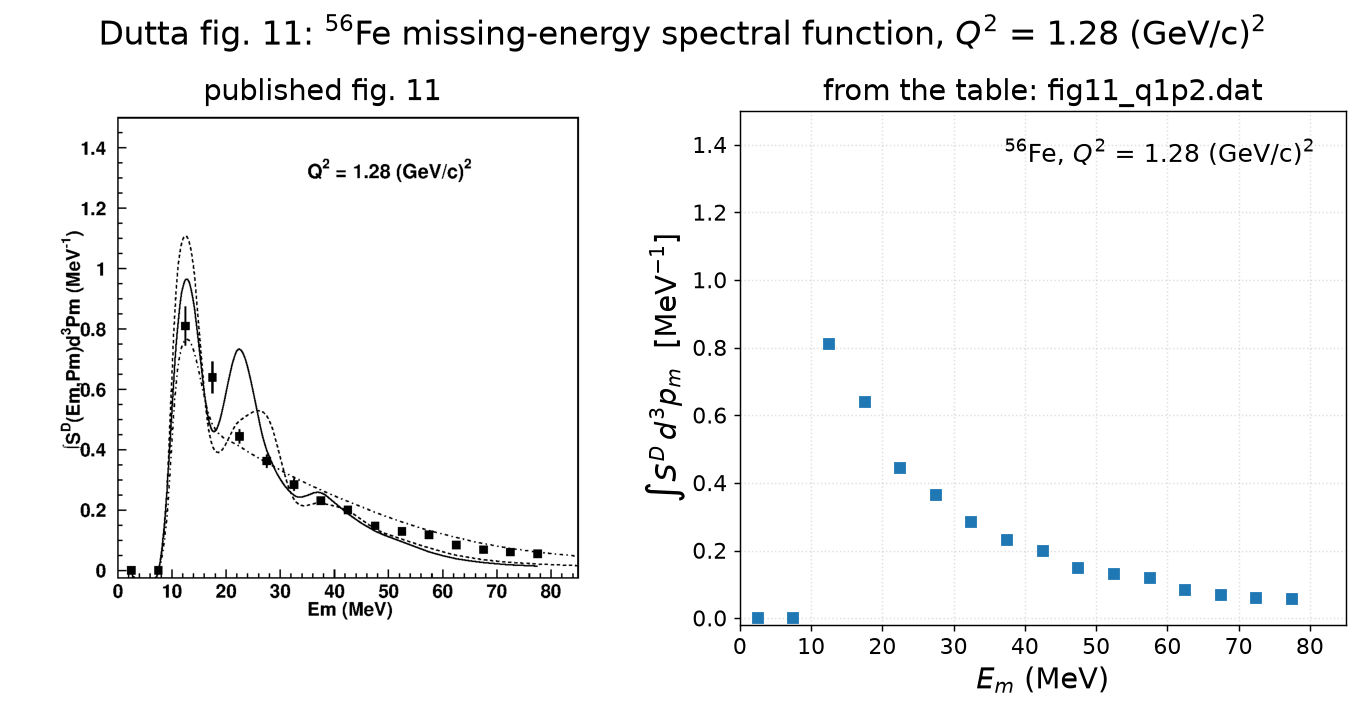
\includegraphics[width=\textwidth]{dutta_fig11_fe56_em_published_vs_table.png}
\caption{Fig.~11 of the paper (left) and the 16 points of \texttt{fig11\_q1p2.dat} (right).}
\end{figure}

\paragraph{\texorpdfstring{$^{56}$Fe}{Fe56} missing momentum (fig~7).}
All four files coincide as printed: median ratios to the $Q^2 = 1.8$
reference 1.17 (0.64), 1.09 (1.28), 1.08 (3.25), signed-axis sums equal to
within 5\,\% (the caption's normalization). No fig~6-type anomaly here.
Bin-wise statistical errors are 1--5\,\%, largest at $|p_m| = 20$ and
300 MeV/c.

\begin{figure}[htbp]
\centering
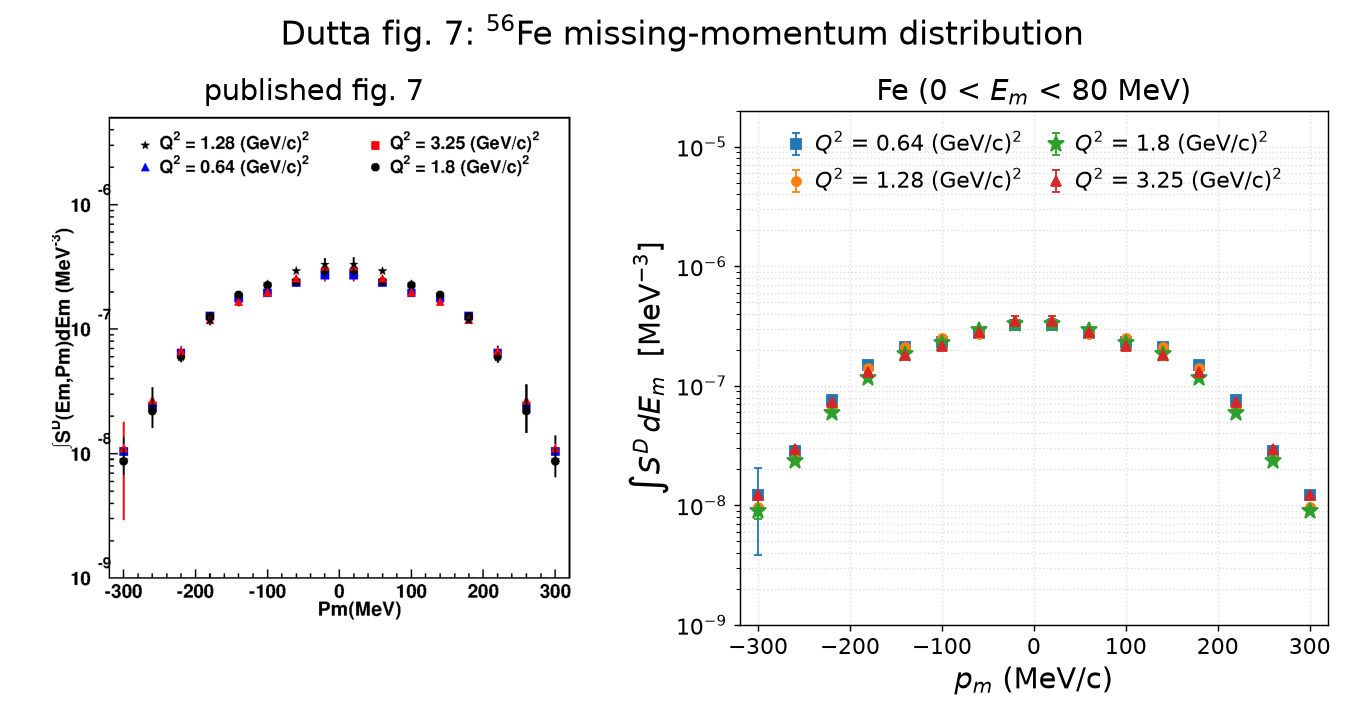
\includegraphics[width=\textwidth]{dutta_fig7_fe56_pm_published_vs_table.png}
\caption{Fig.~7 of the paper (left) and the four \texttt{fig7\_*.dat} files (right).}
\end{figure}
\FloatBarrier

\subsection{Reproduce}

From the repo root:
\begin{verbatim}
pixi run python report/dutta-integral/make_published_vs_table.py
# -> figures/dutta_fig{9,6,11,7}_*_published_vs_table.png
#    figures/dutta_published_vs_table.txt
pixi run python report/dutta-integral/make_report_tex.py      # -> dutta-integral.tex
cd report/dutta-integral && pixi run \
    --manifest-path /exp/dune/data/users/liangliu/texenv/pixi.toml \
    tectonic --outdir . dutta-integral.tex                    # -> dutta-integral.pdf
\end{verbatim}
The script reads the \texttt{.dat} files directly, uses the house plot style
(\texttt{results/template/plot\_style.py}) and writes its histdiag readout with
\texttt{results/template/histdiag.py}; the published renders come from
\texttt{papers/nucl-ex\_0303011/figures/}.

\section{Missing energy at \texorpdfstring{$Q^2 = 1.28$ (GeV/c)$^2$}{Q2 = 1.28 (GeV/c)2}: the tabulated points and their sums}

\subsection{\texorpdfstring{$^{12}$C}{C12} (fig~9)}

The 16 rows of \texttt{fig9\_q1p2.dat} (column~1 = bin centre, column~2 =
$S(E_m)$ as plotted):

\begin{center}
\begin{tabular}{rrr}
\toprule
bin & $E_m$ (MeV) & $S(E_m)$ (MeV$^{-1}$) \\
\midrule
1 & 2.5 & 0.00000 \\
2 & 7.5 & 0.00000 \\
3 & 12.5 & 0.00000 \\
4 & 17.5 & 0.57130 \\
5 & 22.5 & 0.26883 \\
6 & 27.5 & 0.05668 \\
7 & 32.5 & 0.06362 \\
8 & 37.5 & 0.07718 \\
9 & 42.5 & 0.06606 \\
10 & 47.5 & 0.05315 \\
11 & 52.5 & 0.02708 \\
12 & 57.5 & 0.01514 \\
13 & 62.5 & 0.00608 \\
14 & 67.5 & 0.00436 \\
15 & 72.5 & 0.00359 \\
16 & 77.5 & 0.00297 \\
\midrule
\textbf{sum} & & \textbf{1.21604} \\
\bottomrule
\end{tabular}
\end{center}

Sums over the 16 points (errors: column~4 in quadrature, statistical only):

\begin{center}
\begin{tabular}{ll}
\toprule
quantity & value \\
\midrule
$\sum S(E_m)$, plain sum of the tabulated values & $\mathbf{1.21604 \pm 0.00578}$ MeV$^{-1}$ \\
$\sum S(E_m)\,\Delta E$ with $\Delta E = 5$ MeV (the plotted area, 0--80 MeV) & $\mathbf{6.0802 \pm 0.0289}$ \\
$\tfrac12 \sum S(E_m)\,\Delta E$ & $3.0401 \pm 0.0145$ \\
\bottomrule
\end{tabular}
\end{center}

Where the strength sits: the two p-shell bins at 17.5 and 22.5 MeV carry
69.1\,\% of the sum, the four s-shell bins 30--50 MeV carry 21.4\,\%, the dip
bin at 27.5 MeV 4.7\,\% and the tail above 50 MeV 4.9\,\%. The author's
integral for this figure is \textbf{3.04}, i.e.\ half of
$\sum S(E_m)\,\Delta E$; why the plotted area is twice the nucleon count (the
signed $-300 \ldots +300$ MeV/c $p_m$ axis) is the subject of section~3.

Reproduce (the plotted sum and its half are the \texttt{plotted sum} and
\texttt{N} columns):
\begin{verbatim}
pixi run python report/dutta-integral/integrate_dutta.py --files fig9_q1p2
\end{verbatim}

\subsection{\texorpdfstring{$^{56}$Fe}{Fe56} (fig~11)}

The 16 rows of \texttt{fig11\_q1p2.dat} (column~1 = bin centre, column~2 =
$S(E_m)$ as plotted):

\begin{center}
\begin{tabular}{rrr}
\toprule
bin & $E_m$ (MeV) & $S(E_m)$ (MeV$^{-1}$) \\
\midrule
1 & 2.5 & 0.00000 \\
2 & 7.5 & 0.00000 \\
3 & 12.5 & 0.80983 \\
4 & 17.5 & 0.63965 \\
5 & 22.5 & 0.44406 \\
6 & 27.5 & 0.36284 \\
7 & 32.5 & 0.28453 \\
8 & 37.5 & 0.23175 \\
9 & 42.5 & 0.20011 \\
10 & 47.5 & 0.14872 \\
11 & 52.5 & 0.13002 \\
12 & 57.5 & 0.11820 \\
13 & 62.5 & 0.08474 \\
14 & 67.5 & 0.06965 \\
15 & 72.5 & 0.06070 \\
16 & 77.5 & 0.05527 \\
\midrule
\textbf{sum} & & \textbf{3.64006} \\
\bottomrule
\end{tabular}
\end{center}

Sums over the 16 points (errors: column~4 in quadrature, statistical only):

\begin{center}
\begin{tabular}{ll}
\toprule
quantity & value \\
\midrule
$\sum S(E_m)$, plain sum of the tabulated values & $\mathbf{3.64006 \pm 0.01579}$ MeV$^{-1}$ \\
$\sum S(E_m)\,\Delta E$ with $\Delta E = 5$ MeV (the plotted area, 0--80 MeV) & $\mathbf{18.2003 \pm 0.0790}$ \\
$\tfrac12 \sum S(E_m)\,\Delta E$ & $9.1001 \pm 0.0395$ \\
\bottomrule
\end{tabular}
\end{center}

Where the strength sits: the three bins 10--25 MeV carry 52.0\,\% of the sum,
25--50 MeV 33.7\,\%, and the tail 50--80 MeV 14.2\,\% (the last bin alone
1.5\,\%), against 4.9\,\% above 50 MeV for carbon. No author-quoted integral
exists for this figure; the same $\tfrac12$ convention as for fig~9 gives
9.10, to be cross-checked against the fig~7 momentum-distribution integral in
section~4.

Reproduce:
\begin{verbatim}
pixi run python report/dutta-integral/integrate_dutta.py --files fig11_q1p2
\end{verbatim}

\section{Missing momentum at \texorpdfstring{$Q^2 = 1.28$ (GeV/c)$^2$}{Q2 = 1.28 (GeV/c)2}: the tabulated points and their integrals}

The $p_m$ files are tabulated on the signed axis, 16 bins of
$\Delta p = 40$ MeV/c centred at $-300 \ldots +300$ MeV/c, and every file is
exactly left--right symmetric, $y(-p_m) \equiv y(+p_m)$ to full precision.
Two integrals are quoted per file:
\begin{itemize}
\item \textbf{the plotted area} $\sum S(p_m)\,\Delta p$ over all 16 signed
  bins (MeV$^{-2}$) --- the quantity the paper's rescale-to-$Q^2 = 1.8$
  caption equalizes;
\item \textbf{the 3D integral} $N = 4\pi \sum_{p_m > 0} S(p_m)\,p_m^2\,\Delta p$
  over the \textbf{positive half only} ($p_m$ at the bin centre, rectangle
  rule), dimensionless --- the number of protons in the file's $E_m$ window.
  Summing both halves would count each $|p_m|$ twice, since the files are
  symmetrized.
\end{itemize}
Errors are column~4 in quadrature (statistical only). All numbers are the
\texttt{plotted sum} / \texttt{N} columns of \texttt{integrate\_dutta.py}.

\subsection{\texorpdfstring{$^{12}$C}{C12} (fig~6, p-shell and s-shell windows)}

The 16 rows of \texttt{fig6\_top\_q1p2.dat} (p-shell window) and
\texttt{fig6\_bot\_q1p2.dat} (s-shell window), column~1 = bin centre, column~2 =
$S(p_m)$ as plotted, with the per-bin 3D weights ($\Delta p = 40$ MeV/c, $p_m$
at the bin centre). As for iron, the $2\pi$ column summed over all 16 signed
bins is the 3D integral $N$ and the $4\pi$ column over all 16 bins is twice
that.

\needspace{22\baselineskip}
\paragraph{p-shell window, $10 < E_m < 25$ MeV.}
\begin{center}\small\renewcommand{\arraystretch}{0.95}
\begin{tabular}{rrrrr}
\toprule
bin & $p_m$ (MeV/c) & $S(p_m)$, p-shell (MeV$^{-3}$) & $4\pi\,S(p_m)\,p_m^2\,\Delta p$ & $2\pi\,S(p_m)\,p_m^2\,\Delta p$ \\
\midrule
1 & $-300$ & $1.31822\times10^{-9}$ & 0.0596 & 0.0298 \\
2 & $-260$ & $4.15417\times10^{-9}$ & 0.1412 & 0.0706 \\
3 & $-220$ & $1.13985\times10^{-8}$ & 0.2773 & 0.1387 \\
4 & $-180$ & $2.61633\times10^{-8}$ & 0.4261 & 0.2130 \\
5 & $-140$ & $4.86048\times10^{-8}$ & 0.4789 & 0.2394 \\
6 & $-100$ & $5.89047\times10^{-8}$ & 0.2961 & 0.1480 \\
7 & $-60$ & $4.55982\times10^{-8}$ & 0.0825 & 0.0413 \\
8 & $-20$ & $1.81916\times10^{-8}$ & 0.0037 & 0.0018 \\
9 & $+20$ & $1.81916\times10^{-8}$ & 0.0037 & 0.0018 \\
10 & $+60$ & $4.55982\times10^{-8}$ & 0.0825 & 0.0413 \\
11 & $+100$ & $5.89047\times10^{-8}$ & 0.2961 & 0.1480 \\
12 & $+140$ & $4.86048\times10^{-8}$ & 0.4789 & 0.2394 \\
13 & $+180$ & $2.61633\times10^{-8}$ & 0.4261 & 0.2130 \\
14 & $+220$ & $1.13985\times10^{-8}$ & 0.2773 & 0.1387 \\
15 & $+260$ & $4.15417\times10^{-9}$ & 0.1412 & 0.0706 \\
16 & $+300$ & $1.31822\times10^{-9}$ & 0.0596 & 0.0298 \\
\midrule
\textbf{sum, all 16 bins} & & \textbf{$4.28667\times10^{-7}$} & \textbf{3.5306} & \textbf{1.7653} \\
\bottomrule
\end{tabular}
\end{center}

\needspace{22\baselineskip}
\paragraph{s-shell window, $30 < E_m < 50$ MeV.}
\begin{center}\small\renewcommand{\arraystretch}{0.95}
\begin{tabular}{rrrrr}
\toprule
bin & $p_m$ (MeV/c) & $S(p_m)$, s-shell (MeV$^{-3}$) & $4\pi\,S(p_m)\,p_m^2\,\Delta p$ & $2\pi\,S(p_m)\,p_m^2\,\Delta p$ \\
\midrule
1 & $-300$ & $7.38319\times10^{-10}$ & 0.0334 & 0.0167 \\
2 & $-260$ & $1.29075\times10^{-9}$ & 0.0439 & 0.0219 \\
3 & $-220$ & $3.29055\times10^{-9}$ & 0.0801 & 0.0400 \\
4 & $-180$ & $7.72794\times10^{-9}$ & 0.1259 & 0.0629 \\
5 & $-140$ & $1.72738\times10^{-8}$ & 0.1702 & 0.0851 \\
6 & $-100$ & $3.00671\times10^{-8}$ & 0.1511 & 0.0756 \\
7 & $-60$ & $4.34589\times10^{-8}$ & 0.0786 & 0.0393 \\
8 & $-20$ & $5.10294\times10^{-8}$ & 0.0103 & 0.0051 \\
9 & $+20$ & $5.10294\times10^{-8}$ & 0.0103 & 0.0051 \\
10 & $+60$ & $4.34589\times10^{-8}$ & 0.0786 & 0.0393 \\
11 & $+100$ & $3.00671\times10^{-8}$ & 0.1511 & 0.0756 \\
12 & $+140$ & $1.72738\times10^{-8}$ & 0.1702 & 0.0851 \\
13 & $+180$ & $7.72794\times10^{-9}$ & 0.1259 & 0.0629 \\
14 & $+220$ & $3.29055\times10^{-9}$ & 0.0801 & 0.0400 \\
15 & $+260$ & $1.29075\times10^{-9}$ & 0.0439 & 0.0219 \\
16 & $+300$ & $7.38319\times10^{-10}$ & 0.0334 & 0.0167 \\
\midrule
\textbf{sum, all 16 bins} & & \textbf{$3.09754\times10^{-7}$} & \textbf{1.3868} & \textbf{0.6934} \\
\bottomrule
\end{tabular}
\end{center}

\begin{center}\small
\begin{tabular}{lll}
\toprule
quantity & p-shell window & s-shell window \\
\midrule
$\sum S(p_m)$, plain sum (MeV$^{-3}$) & $4.28667\times10^{-7}$ $\pm$ $4.3\times10^{-9}$ & $3.09754\times10^{-7}$ $\pm$ $3.8\times10^{-9}$ \\
$\sum S(p_m)\,\Delta p$, signed axis (MeV$^{-2}$) & $1.7147\times10^{-5}$ $\pm$ $1.7\times10^{-7}$ & $1.2390\times10^{-5}$ $\pm$ $1.5\times10^{-7}$ \\
$4\pi\sum_{p_m>0} S\,p_m^2\,\Delta p$, positive half & $\mathbf{1.7653 \pm 0.0198}$ & $\mathbf{0.6934 \pm 0.0065}$ \\
\bottomrule
\end{tabular}
\end{center}

\needspace{26\baselineskip}
\subsection{\texorpdfstring{$^{56}$Fe}{Fe56} (fig~7, full 0--80 MeV window)}

The 16 rows of \texttt{fig7\_q1p2.dat}, with the per-bin 3D weights
($\Delta p = 40$ MeV/c, $p_m$ at the bin centre): the $2\pi$ column summed
over all 16 signed bins is the 3D integral $N$; the $4\pi$ column over all 16
bins is twice that, since the file is symmetric and each $|p_m|$ appears on
both sides:

\begin{center}\small\renewcommand{\arraystretch}{0.95}
\begin{tabular}{rrrrr}
\toprule
bin & $p_m$ (MeV/c) & $S(p_m)$ (MeV$^{-3}$) & $4\pi\,S(p_m)\,p_m^2\,\Delta p$ & $2\pi\,S(p_m)\,p_m^2\,\Delta p$ \\
\midrule
1 & $-300$ & $9.66999\times10^{-9}$ & 0.4375 & 0.2187 \\
2 & $-260$ & $2.45150\times10^{-8}$ & 0.8330 & 0.4165 \\
3 & $-220$ & $6.71838\times10^{-8}$ & 1.6345 & 0.8172 \\
4 & $-180$ & $1.41263\times10^{-7}$ & 2.3006 & 1.1503 \\
5 & $-140$ & $2.10452\times10^{-7}$ & 2.0734 & 1.0367 \\
6 & $-100$ & $2.52322\times10^{-7}$ & 1.2683 & 0.6342 \\
7 & $-60$ & $2.69957\times10^{-7}$ & 0.4885 & 0.2443 \\
8 & $-20$ & $3.33847\times10^{-7}$ & 0.0671 & 0.0336 \\
9 & $+20$ & $3.33847\times10^{-7}$ & 0.0671 & 0.0336 \\
10 & $+60$ & $2.69957\times10^{-7}$ & 0.4885 & 0.2443 \\
11 & $+100$ & $2.52322\times10^{-7}$ & 1.2683 & 0.6342 \\
12 & $+140$ & $2.10452\times10^{-7}$ & 2.0734 & 1.0367 \\
13 & $+180$ & $1.41263\times10^{-7}$ & 2.3006 & 1.1503 \\
14 & $+220$ & $6.71838\times10^{-8}$ & 1.6345 & 0.8172 \\
15 & $+260$ & $2.45150\times10^{-8}$ & 0.8330 & 0.4165 \\
16 & $+300$ & $9.66999\times10^{-9}$ & 0.4375 & 0.2187 \\
\midrule
\textbf{sum, all 16 bins} & & \textbf{$2.61842\times10^{-6}$} & \textbf{18.2057} & \textbf{9.1029} \\
\bottomrule
\end{tabular}
\end{center}

\begin{center}\small
\begin{tabular}{ll}
\toprule
quantity & value \\
\midrule
$\sum S(p_m)$, plain sum (MeV$^{-3}$) & $2.61842\times10^{-6}$ $\pm$ $2.4\times10^{-8}$ \\
$\sum S(p_m)\,\Delta p$, signed axis (MeV$^{-2}$) & $1.0474\times10^{-4}$ $\pm$ $9.4\times10^{-7}$ \\
$4\pi\sum_{p_m>0} S\,p_m^2\,\Delta p$, positive half & $\mathbf{9.1029 \pm 0.0498}$ \\
\bottomrule
\end{tabular}
\end{center}

Reproduce:
\begin{verbatim}
pixi run python report/dutta-integral/integrate_dutta.py \
    --files fig6_top_q1p2 fig6_bot_q1p2 fig7_q1p2
\end{verbatim}

\end{document}
